\begin{figure}[htb]
    \centering
    \caption{Correlation Between Median Rent Price (in dollars per square foot) and previous year change in MW (percentage).}
    \scalebox{0.20}{
    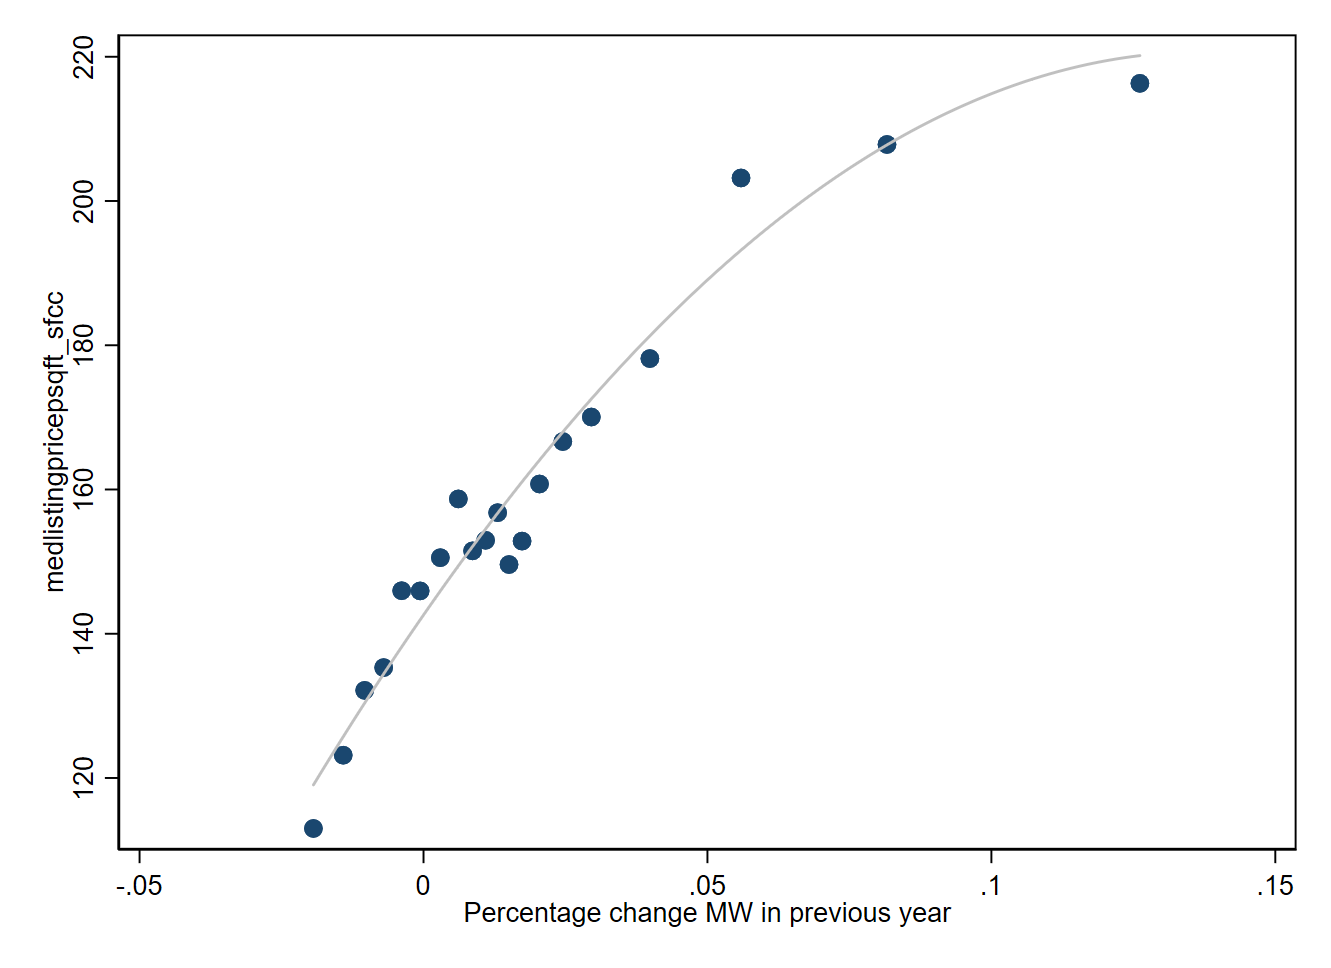
\includegraphics{draft_june20/tempfigure/binsc_medlistingpricepsqft_sfcc_pctMWch.png}}
    \subcaption*{\textit{Note}: The figure presents the correlation between median listing price on Zillow.com at the zipcode-year level and the percentage change in MW in the previous year. Data comes from the final sample used in the analysis (see \autoref{sec:data} for more details). Each zipcode yearly observation is obtained by averaging monthly observations, the basic time unit in this paper. The correlation is taken after controlling for year fixed effects, resident population, urban share, median income, black population share, and number of housing units.All demographic characteristics come from the 2010 Census.   
    }
    \label{appfig:binsc_listing_mwpctchange}
\end{figure}

\begin{figure}[h!]
    \centering
    \caption{Effects of a MW change on single family houses and condos rent per square foot (in dollars) for different definition of MW change event.}
    \scalebox{1}{
        \begin{subfigure}[b]{.5\linewidth}
            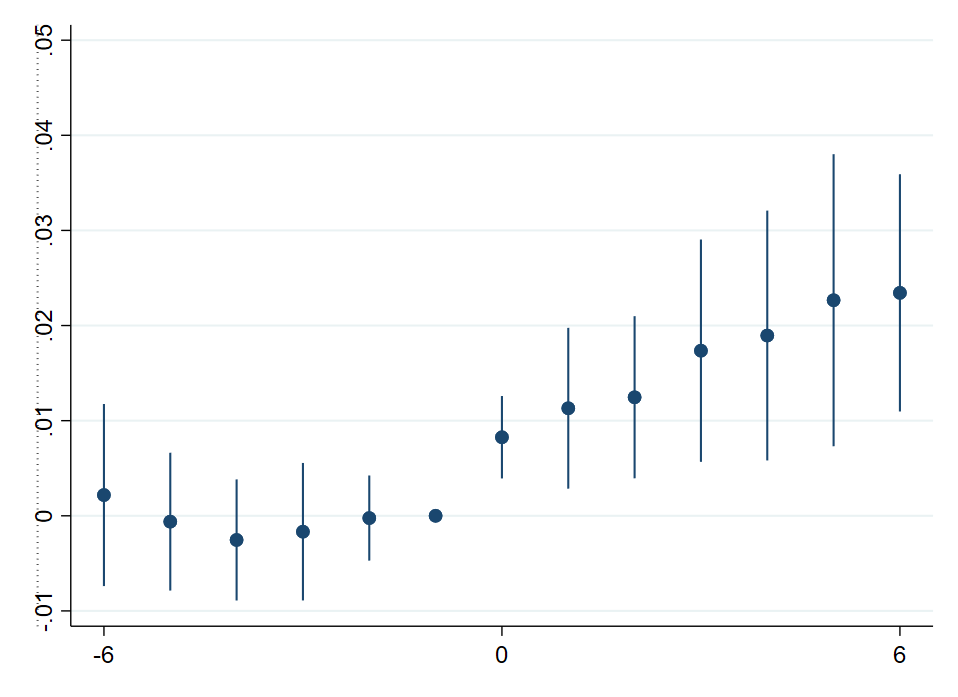
\includegraphics[width=\linewidth]{analysis/event_size_robustness/output/last_rentpsqft_sfcc_event025_w6.png}
            \caption{Mw changes of at least $\%0.25$}
        \end{subfigure}
        \quad 
        \begin{subfigure}[b]{.5\linewidth}
            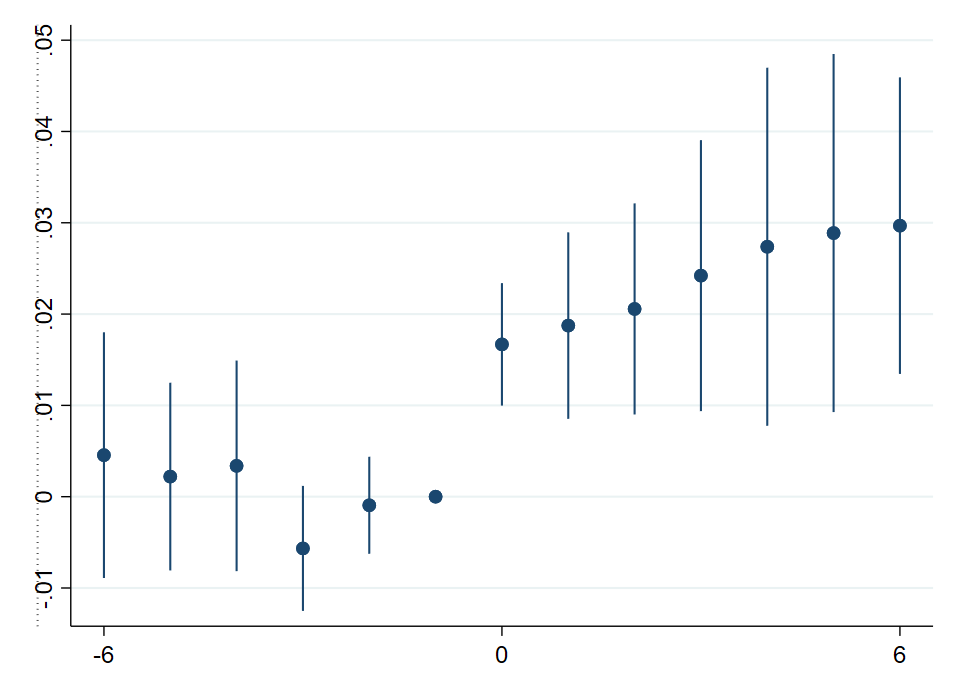
\includegraphics[width=\linewidth]{analysis/event_size_robustness/output/last_rentpsqft_sfcc_event075_w6.png}
            \caption{Mw changes of at least $\%0.75$}
        \end{subfigure}
    }
    \subcaption*{\textit{Note}: The figure shows the estimated $\hat{\delta}_{t+k}$ coefficients from the baseline specification (\autoref{eq:main_ziplevel}) for different events. In panel (a) we select all MW changes of at least $\$0.25$; in panel (b) we focus on all MW changes of at least $\$0.75$. For each zipcode, we  add the sum of unused events and county-level seasonality as additional controls ($X_{jt}$). Standard errors are clustered at the zipcode level.}
    \label{appfig:event_level_robustness6}
\end{figure}